\chapter{Evolution de l'interdiction du \riba et \gharar}
%{\Large\textbf{Evolution de l'interdiction du \riba et \gharar}}
\mn{Guillaume Gorge - ISTR 2022 - Courants de l'Islam Contemporain}


\section{Introduction}

En tant que membre du jury d'admission de l'Institut des Actuaires, j'ai eu à me prononcer sur certains mémoires présentés par des étudiants sur la \textit{finance Islamique} et \textit{l'assurance Takaful}. Ces mémoires ne couvrent pas les présupposés théologiques et commencent généralement par une présentation des interdits de la loi musulmane, comme par exemple ce \href{http://www.ressources-actuarielles.net/EXT/ISFA/1226-02.nsf/0/8c814ff5f2bae57ec1257e1a004407b6/\%24FILE/Memoire_ISFA_Tontines_et_Takaful_Bendimerad_Version_avec_Couverture.pdf}{mémoire d'actuariat} : 
\begin{quote}
     [pour faire face à ses  engagements, l'assureur],peut, par exemple, inclure des actifs obligataires dont les taux de rendement font apparaître des taux d'intérêt. [...] l'interdiction de l'usage du taux d'intérêt, appelé \textit{\riba} en arabe, est l'un des fondements du droit des affaires musulman. \sn{\cite{Actuariat:Takaful}}
\end{quote}
Dans la même veine, sont généralement définis les autres interdits, comme le \gharar, défini dans le même mémoire comme : 
\begin{quote}
    Le contrat d'assurance peut constituer une perte disproportionnée en faveur de l'un des participants aux dépens de l'autre. Ce caractère d'incertitude, appelé \gharar en arabe, est un caractère prohibé par l'Islam surtout lorsque le transfert du risque vers un tiers est total, ce qui est notamment le cas pour l'assureur qui porte entièrement la charge du risque cédé par l'assuré. \sn{\cite{Actuariat:Takaful}}
\end{quote}


Connaissant les travaux d'Averroes et la science de la chance\sn{d'où dériverait le mot hasard} , j'ai été intrigué par cette apparente clarté de l'interdiction par l'Islam de l'\textit{intérêt} et de \textit{l'incertitude}, deux concepts qui sont pourtant à la base de l'économie moderne, je me propose d'étudier l'évolution de l'opposition du {\riba} et\gharar dans les différents courants de l'Islam contemporain, depuis la pensée d'Abduh. 

\paragraph{l'enjeu du \riba et du \gharar}
A travers les mémoires d'actuariat consultés qui essayent de dépasser de trouver des solutions (souvent complexes pour le client) respectant ces interdictions, on peut déceler une tension réelle entre la réalité rencontrée par l'actuaire musulman et ce qu'en dit l'Islam : 
\begin{quote}
     
A l'issue de l'analyse précédente, l'idée même d'une assurance islamique semble être un contresens. Pourtant, la religion musulmane encourage l'individu à prendre des mesures pour réduire l'ampleur des désastres qui pourraient l'affecter. D'après un Hadith authentifié, le prophète conseille à un croyant de placer sa confiance en Dieu et d'attacher son chameau plutôt que de se limiter uniquement à placer sa confiance en Dieu en offrant la possibilité au chameau libre de s'échapper. L'Islam ne s'oppose donc pas à l'idée de vouloir minimiser les risques et par conséquent elle ne s'oppose pas à faire usage de la loi des grands nombres. Elle exclut certes la spéculation et l'incertitude ainsi que le taux d'intérêt. En revanche, elle compte parmi ses principes la coopération et l'entre-aide mutuelle ainsi que le partage équitable des risques et des bénéfices.\sn{\cite{Actuariat:Takaful}}
\end{quote}




L'interdiction des deux notions n'a pas la même importance économique ni la même force juridique et l'interdiction du {\riba} a donné lieu à plus de développements. En partant de ces études, j'essayerais néanmoins de transposer ces travaux à l'assurance.
Après avoir étudié la façon dont les penseurs de l'Islam contemporains répondent à cette question que pose l'économie moderne, je proposerai quelques pistes sur le propre cheminement du Christianisme sur ces questions. Après tout, le prêt à intérêt était aussi interdit au Moyen-äge en Europe. Ces pistes seront en particulier nourries par la présentation de la pensée de Saint Thomas d'Aquin sur les taux d'intérêt et comment ces pistes peuvent nourrir la réflexion de la théologie musulmane (et chrétienne) contemporaine. 
 

%---------------------------------------------------------------------------------------------------------------
\section{Vision dans l'Islam Classique de l'interdiction du \riba}

\subsection{une interdiction du \riba et \gharar}

Pour commencer, il est utile de se référer aux textes à l'origine de ces interdits.
\paragraph{Versets du Coran et Hadiths interdisant le \riba}
Le verset 130 de la Sourate 3, Al-Imran mentionne : 
\vocalize % switch diacritics for short vowels on
\transtrue % display the transliteration
\arabtrue % print arabic text (on by default)
\begin{quote}
 
\TArabe{
 يَا أَيُّهَا الَّذِينَ آمَنُوا لَا تَأْكُلُوا الرِّبَا أَضْعَافًا مُّضَاعَفَةً وَاتَّقُوا اللَّهَ لَعَلَّكُمْ تُفْلِحُونَ
  } 
O vous qui croyez !, ne vivez pas du {\riba} [produisant le] double deux fois ! Soyez pieux envers Allah ! Peut-être serez-vous bienheureux. 

\end{quote}
Par ailleurs, les versets 278 et 279 de la sourate 2, Al-Baqara :
\begin{quote}
\begin{flushright}    
\TArabe{
 يَا أَيُّهَا الَّذِينَ آمَنُوا اتَّقُوا اللَّهَ وَذَرُوا مَا بَقِيَ مِنَ الرِّبَا إِن كُنتُم مُّؤْمِنِينَ
فَإِن لَّمْ تَفْعَلُوا فَأْذَنُوا بِحَرْبٍ مِّنَ اللَّهِ وَرَسُولِهِ وَإِن تُبْتُمْ فَلَكُمْ رُءُوسُ أَمْوَالِكُمْ لَا تَظْلِمُونَ وَلَا تُظْلَمُونَ
} 
\end{flushright}    

 O vous qui croyez !, soyez pieux envers Allah ! Faites abandon de ce qui [vous] reste [à toucher provenant] du {\riba}, si vous êtes croyants !
 Si vous ne le faites point, attendez-vous à une guerre de la part d’Allah et de Son Apôtre ! si vous vous repentez, alors vous récolterez votre capital sans infliger ou être victime d’une injustice. \sn{Traduction de Blachière, sauf la dernière phrase {\cite{ElGamal:BanqueFinanceIslamique}}}

\end{quote}

De même, un hadith de Abu Hurayra met au même niveau la \textit{\riba} et le meurtre : 
\begin{quote}
    "Evitez les sept turpitudes !"

- "Quelles sont-elles, ô Envoyé d'Allah?", demandèrent les fidèles.

- "Ce sont, répondit-il : le polythéisme, la magie, le meurtre qu'Allah a interdit sauf à bon droit, l'usurpation des biens de l'orphelin, le \textit{\riba}, la fuite du front au jour du djihad et la fausse accusation (de fornication) des femmes vertueuses, chastes et croyantes".
\end{quote}
 
  Nous avons évité à ce stade de traduire le terme de \textit{\riba}, par \textit{usure} ou \textit{intérêt}. Le Hadith rapport par at-Tirmidhî a été utilisé pour appliquer le sens d'intérêt à la \textit{\riba}  : 
 \begin{quote}
     Vendez de l'or contre de l'argent (les quantités échangées étant) comme vous voulez, à condition que ce soit main à main. Vendez du blé contre des dattes sèches (les quantités échangées étant) comme vous voulez, à condition que ce soit main à main. Vendez de l'orge contre des dattes sèches (les quantités échangées étant) comme vous voulez, à condition que ce soit main à main (n° 1240)
 \end{quote}  
 On peut effectivement y lire le refus de l'intérêt mais d'autres lectures sont possibles, en particulier en relevant l'insistance du hadith à une transaction \textit{main à main}, qui permet une transaction claire. Par ailleurs, la valeur du temps n'est pas explicitement mentionnée.
 
\paragraph{Indulgence vis à vis du \gharar}

Les juristes ont été plus indulgents, à divers degrés, par rapport à l’interdiction du \gharar étant donné qu’aucun contrat ne peut être totalement dépourvu d’incertitude. 
Comme le \riba, le \gharar est lié aux contrats de vente à terme. Il se définit comme manque de certitude contractuelle et à ce titre doit être évité. Les jurisconsultes classiques \sn{\cite{Rittenberg:Gharar}} ont essayé de définir cette \textit{incertitude}, concept par essence négatif, par un cadre juridique le plus objectif possible. En pratique, ils ont étudié les biens présentant le plus d'hétérogénéité et donc d'incertitude lors d'une vente à terme (ex : un cheval de course interdit à la vente à terme). 
 
\subsection{Un contexte liés aux contrats profondément différents des débuts de l'Islam}
Si l'on suit Lindbeck, la pertinence religieuse peut se juger par  
\begin{quote}
     [...] sa capacité à fournir dans ses propres termes une interprétation intelligible des diverses situations et réalités que rencontrent ses adhérents. Les religions que nous qualifions de primitives échouent régulièrement à ce test quand elles sont confrontées à des changements importants, tandis que les religions mondiales développent de plus grandes ressources pour faire face aux vicissitudes \sn{\cite[175]{Lindbeck:NatureDoctrineFr} } 
\end{quote}

Or, il faut reconnaître que la pratique des contrats aujourd'hui est bien différente de celle de l'époque du Prophète : Avec l'accumulation des richesses dans les villes italiennes au moyen-âge naît le capitalisme et la finance : comment financer et assurer les bateaux partant de Gênes et remplis de richesse ? Cette irruption de la finance pose de nouvelles questions, à commencer historiquement au Christianisme. Les réponses furent plurielles, entre une vie de pauvreté proposée par Saint François d'Assise ou la réflexion de l'université de Paris et de Saint Thomas d'Aquin sur la notion d'usure et de juste prix. 
L'économie moderne souligne que du point de vue du prêteur, le prêt a un prix du fait du risque  de défaut de l'emprunteur et de la valeur temps (qui correspond principalement à l'inflation). La pertinence économique de l'intérêt et de la prise de risque est donc justifiée même si cela ne veut pas dire qu'elle l'est d'un point de vue religieux.
Ces nouvelles questions touchèrent plus tardivement le monde musulman, au XIXè, avec l'arrivée simultanée de l'industrialisation, qui nécessite des capitaux importants et les débuts de la colonisation. Par l'industrialisation, le capital permet une forte augmentation des capacités productives, mais aussi la concentration des risques qui ne peuvent être portée par la solidarité traditionnelle : d'où la naissance des banques et assurances au XIXè.
Face à ces nouvelles questions, quelles sont les réponses proposées par les théologiens musulmans ?




%---------------------------------------------------------------------------------------------------------------
\section{Éléments théologiques apportés}

\subsection{Premières réponses face à la nécessité du prêt et de l'assurance}
\paragraph{Le développement du \riba et de l'assurance par les Occidentaux} Les prêts à intérêt ont toujours existé au sein de l'Empire Ottoman \sn{\cite{Gilbar:Qadi}}, principalement portés par des familles grecques, arméniennes ou juives (et en Iran par les arméniens et zoroastriens). A ce premier groupe, s'ajouta les banques commerciales européennes ou les banques "étrangères-locales" comme la banque impériale ottomane au XIXè.
De la même façon pour les assurances, Ibn Abidin, représentant de l'école officielle de droit Hanadi dans l'empire ottoman, suggère le compromis suivant : il est licite d'établir des contrats d'assurance portant sur les risques encourus à l'intérieur du royaume islamique -le Dar al Islam- à condition que ces contrats soient conclus avec une compagnie d'assurance ayant son siège hors de pays de l'Islam. 

\paragraph{Utilisation de prêt à intérêt par les musulmans} L'interdiction du {\riba} a pu poser des problèmes pour les grands marchands arabes (tujjār).  
Pour l'école Hanafite, le terme de \riba peut être traduit par usure, dans le sens d'un taux d'intérêt exorbitant, à l'opposé de l'intérêt raisonnable, le \emph{ribh}. L'autre interprétation dominante, attribuée à 'Abdahallah Ibn 'Abbas, permet d'expliquer la notion du Coran de double capital par la pratique du \textit{\riba al jâhiliyya} (préislamique), avec des taux d'intérêt très élevés avec des intérêts pouvant dépasser le capital en cas de non-paiement. A l'opposé de ces analyses plus ouvertes, la position de l'école Hanbalite fut l'interdiction pure de l'intérêt. Pour contourner l'interdit de l'interdit de l'école Hanbalite du \riba face à la nécessité, les marchands musulmans mirent en place des montages complexes où l'intérêt était déguisé en une \textit{double vente} (\emph{mukhâtra}) avec deux ventes fictives successives permises par la \textit{sha'ia}: 
\begin{itemize}
    \item la première, le préteur vent un objet à l'emprunteur pour une somme équivalente au capital et à l'intérêt. l'emprunteur s'engage à payer la valeur de l'objet à la fin de la période (techniquement, une vente avec paiement différé). 
    \item A la fin de cette première transaction, l'emprunteur revend le même objet pour la valeur du principal (techniquement, une vente à terme).
\end{itemize}
 Cependant,  au moyen-orient entre le XVIè et le XVIIIè siècle, des exemptions partielles ou totales de paiement de l'intérêt du fait de son incompatibilité avec l'Islam ont été exigé par les cours de justice religieuses \sn{\cite{Gilbar:Qadi}}.
 


\section{la position d'Abduh}
\paragraph{Le Cheikh {Muhammad Abduh} (1849 - 1905)} Cet égyptien, successeur et ami d'Al Afghani, est l'une des figures marquantes du réformisme islamique. Il s'oppose au colonialisme atteignant alors l'Egypte. Son séjour  parisien le convainc de la nécessité de réforme de l'Islam et l'initie aux réflexions intellectuelles occidentales et en particulier François Guizot. Il pense ainsi l'Islam comme civilisation, avec la notion de progrès qui y est lié, et pas uniquement comme Religion. Il n'y a pas d'opposition pour lui entre Foi et Raison, la religion musulmane étant \textit{raisonnable}.   

\subsection{Position du \emph{Rissalat al Tawhid}}
Dans son livre principal, le \emph{Rissalat al Tawhid} {\citep{Abdou:Rissalat}}, Abduh part de la Raison pour montrer le besoin que l'homme ne se fixe pas sa propre loi.

Il montre tout d'abord la naissance des besoins et des liens entre les hommes. Idéalement ces liens seraient ceux de l'amour : 
\begin{quote}
    Nul ne met en doute que chaque membre d'une société a besoin
des autres membres; et chaque fois que l'individu accroître ses exigences
dans la vie il ressent plus fortement le besoin de recourir au concours
de ses semblables. Ainsi se développent les besoins et à leur suite s'étendent
les relations de la famille à la tribu, de celle-ci à la nation, et finalement
au genre humain tout entier, comme le montre notre époque . Ces
besoins qui créent dans le sein de chaque nation (surtout dans le sein de
celles qui méritent vraiment ce nom) des relations et des rapports
spéciaux la distinguant des autres nations, sont le besoin de se procurer
sa subsistance, celui de profiter des biens de la vie, celui d' acquérir
les choses désirables et d'éloigner de soi celles qui déplaisent. 
Si la vie de l'homme se déroulait selon les lois de la nature, telles
que nous les voyons appliquées aux autres êtres vivants, les besoins
que nous venons de citer auraient été parmi les facteurs les plus puissants
de l'amour entre les individus[...].  

[\ldots]
Si par contre, l'intérêt se mêle aux relations amicales, et si chacun des amis exige un prix pour son amour, celui-ce se change en esprit d'exploitation, il se reporte sur l'effet utilitaire et se transforme chez l'un des amis en un abus de la force, et chez l'autre, en peur avilissante, en dissimulation et en hypocrisie.
\sn{\cite[p.66]{Abdou:Rissalat}}
\end{quote}
Mais l'homme ne vie pas selon les lois de la nature car il est inconstant : 
\begin{quote}
 l 'homme
a été créé avec un caractère inconstant; quand le malheur l'atteint
il est abattu, et quand il acquiert quelque bien il devient insolent.
(C. ch. 70, v. 19 à 21). [...]
Chaque fois que la mémoire et l'imagination les poussent à
éviter quelque chose qui leur inspire de la crainte ou à atteindre un
objet qui leur fait envie, leur intelligence leur ouvre une porte de la
ruse ou leur découvre une voie de la violence ; alors le rapt remplace
l'échange pacifique, la dispute prend la place de l'union et la conduite
de l'homme riche s 'appuie plus que sur l'astuce et la violence.
\sn{\cite[p 68]{Abdou:Rissalat}}
\end{quote}
il montre qu'on peut accéder à l'équité par des voies naturelles mais qu'à la fois pour les masses et pour éviter la corruption des élites, il est nécessaire de s'appuyer sur une loi externe.
\begin{quote}
[...] ] le genre humain
a surtout besoin, pour conserver son existence, de l'amour ou d'un
sentiment qui le remplace.
A différentes époques il y a eu des penseurs qui ont fait appel à
l'équité ; ils ont pensé, et même quelques mystiques ont exprimé cette
pensée par de nobles paroles, que l'équité remplace l'amour. Cette
assertion ne manque pas de sagesse, mais qui peut établir les
règles de l'équité et amener la totalité des hommes à se soumettre ?
\sn{\cite[p 69]{Abdou:Rissalat}}
\end{quote}

Suivre la Loi de Dieu, ordonner le bien est alors supérieur à la foi : 

\begin{quote}
  le Coran indique
qu'il n'y a pas de condition meilleure que celle des hommes qui ordonnent
le bien et défendent le mal: \begin{quote}
    Vous êtes les meilleurs parmi les hommes,
vous ordonnez le bien, vous défendez le mal et vous croyez en Dieu. (Cor. ch. 3, v. 106.) 
\end{quote} 
 
Dans ce verset le fait d'ordonner le bien et de
défendre le mal est mentionné avant la foi en Dieu, bien que la foi soit la base même sur laquelle s'appuient les bonnes oeuvres. 
\sn{\cite[p 121]{Abdou:Rissalat}}
\end{quote}

\paragraph{Conséquence pratique pour le \riba}
Abduh liste alors une liste de maux que l'Islam permet d'éviter : 
\begin{quote}

[l'Islam] nous invite par dessus tout à dépenser notre bien pour les oeuvres
charitables et souvent il en fait l'expression de la foi et la manifestation
d'une bonne conduite; il déracina par là, du coeur des pauvres, la rancune
et la haine contre ceux que Dieu a favorisé des biens terrestres ; il leur
inspira l'amour pour les riches, tout comme il fît naître dans le coeur de
ceux-ci la pitié pour les malheureux ; ainsi il développa la confiance dans
le coeur de tous les hommes. Quel remède plus efficace contre les maux
dont souffre la société: «C'est une faveur que Dieu accorde à qui il veut,
car Dieu est d'une bienfaisance sans bornes.» (Cor. ch. 57, v. 21.)
\textsc{L' Islam a fermé les deux portes du mal, il a bouché les deux sources
qui minent l'intelligence et détruisent la richesse, en frappant les boissons
enivrantes, les Jeux de hasard et l'usure, d'une interdiction absolue qui
n'admet pas d'infraction.}
\sn{\cite[p 122]{Abdou:Rissalat}}
\end{quote}
Ainsi, parmi ces maux figure le \riba traduit ici par \textit{usure}.


\subsection{l'avis sur la la Caisse d'Epargne en Egypte}


\paragraph{Un premier cas pratique : l'assurance vie en Egypte}
 La Compagnie d'Assurances al-Chark,
au Caire,  conservait une copie d'une fatwa d'Abduh \textit{écrite initialement pour un particulier} afin de la montrer à ses clients, le cas échéant. Le
client effectue des versements réguliers et périodiques par tranches successives
prévues d'avance ; la compagnie les encaisse et se charge de faire fructifier cet
argent. Finalement, à l'échéance, la société remboursera le total des versements
effectués augmenté des bénéfices résultant de la fructification. La fatwa admet
la licéité d'une telle opération en des termes qui, au fond, s'appliqueraient à toute
société en commandite. Il faut noter que la revue Al-Manâr de \textit{Rashid Rida} ne nia pas l'authenticité de cette fatwa après la mort d'Abduh mais protesta contre l'extension faite à toute assurance vie. On voit néanmoins que la problématique d'un conflit avec le \gharar ne semble pas avoir été mentionnée par Abduh ni Rida dans le contexte des premières assurances en Egypte.

\paragraph{la note de la revue Al-Manâr de 1903 par rapport à la Caisse d'Epargne} Face aux scrupules de 3000 musulmans à toucher les intérêts (fa'ida) de la Caisse d'Eparne, un échange eu lieu entre le directeur et le Cheick Abduh, échange repris par la revue \textit{Al-Manâr}. Abduh y maintenait fermement le principe de
l'interdiction absolue de l'usure et du \riba ; mais il ne classait pas le cas de la Caisse
d'Epargne avec ceux de l'usure. Il l'assimilait à celui d'une société en commandite
(chirkat al-mod'âraba). A la suite de cette discussion, la loi fut modifiée en 1904 : 
 

\begin{quote}
 Il est prévu dans l'article premier que le client devra signer un
formulaire imprimé dans lequel il déclarera donner au Directeur Général de la
Poste tout pouvoir pour faire fructifier les sommes déposées, d'une façon licite et
en excluant toute opération usuraire. Il déclare permettre au Directeur de la Poste
de joindre ses dépôts à ceux des autres clients pour les faire fructifier en commun
à condition de recevoir une part de bénéfices (al-ribh') proportionnelle à ses
versements. On notera que dans cet article comme dans tout le reste de la loi le
mot de \textit{fâ'ida}, intérêt, est totalement absent. \sn{\cite{Jomier:AdbouCaisseEpargne}}
\end{quote}

\begin{quote}
    L'article deux stipule entre autres ce qui suit. Il évite de parler de tant pour
cent, formule qui rappelle trop les intérêts. Il note que la part des bénéfices ne
dépassera pas un pour quarante du capital et le surplus, s'il y en a, reviendra à
l'administration postale à titre de compensation pour les services rendus et les
frais que ceux-ci comportent. L'assimilation à la société en commandite est ainsi
mise en accord avec le fait que la proportion des bénéfices touchés est fixe. On
notera que la proportion de un pour quarante est familière aux oreilles des
musulmans pieux puisque dans un certain nombre de cas le montant de la Zakat
atteint ce chiffre.
\end{quote}


Abduh développe la raison de cette position dans la fatwa et la note du manâr du 18 mars 1904: 
\begin{quote}
    La raison de l'interdiction de l'usure est de faire cesser l'injustice et de conserver les vertus de solidarité et de bonté mutuelle
\end{quote}
On voit donc la position d'Abduh comme ferme dans les principes et ouvert dans l'application, même si cela se traduit par une subtilité juridique. 

\section{L'approche de Rashid Rida sur le \riba}
% - ----------------------------------------
 

Rida est l'un des successeurs spirituels de Abduh. Il fonda avec Abduh la revue néo-réformiste al-Manâr en   1898. Elle définit sa politique éditoriale à l’égard «de la civilisation occidentale» sous forme de deux impératifs : 
\begin{quote}
    \item  1/ Il faut que la terre musulmane puisse rattraper l’Europe sur le plan des sciences modernes, de l’industrie et de l’innovation technique. 
    \item 2/ En contrepartie, il faut déclarer une guerre sans merci à tout ce qui a accompagné l’entrée des Européens en terre musulmane comme décadence morale et mauvaises mœurs
\end{quote}

\paragraph{Une lecture originale du \riba  qui sera ensuite reprise pour fonder l'économie Islamique } Si la position de Rida vis à vis de la liceité de l'intérêt est dans les faits la même que celle d'Abduh, Rida pose son raisonnement par une analyse détaillée des versets du Coran et des Hadiths parlant du \riba  \sn{\cite{Siddique:DemystifyingRiba}}. 
Rida part de l'analyse du mot \riba comme \textit{excès}, et en particulier reprend l'analyse de la sourate 3,125 présentée au début d'un excès lié à la renégociation de la dette. De là, il conclut que ce qui est interdit par le Coran sont les intérêts ajoutés à la fin de la période de prêt (\riba ’l-jahiliyyah). D'une certaine façon, ce sont les intérêts composés ("intérêt d'intérêt") qui sont interdits, ce qui arrive en cas de non paiement à la fin de la période définie. Cette distinction permet à Rida d'autoriser les intérêts bancaires. Il ne sera cependant pas suivi sur ce point par la majorité des jurisconsultes qui étendront l'interdiction du \riba du Coran à tout intérêt, simple ou composé (intérêt d'intérêt). En revanche, ces derniers adopteront sa distinction entre les différents \riba du Coran et du Hadith. Mais cette distinction, loin de simplifier le sujet, rend les discussion assez techniques, en particulier parce que les différentes écoles appliquent aux hadiths des méthodes d'analyse différentes que celles appliquées sur le Coran. 
 

 \section{Une lecture plus restrictive du \riba}
\paragraph{Les frères musulmans} L'exemple du \riba montre la capacité d'adaptation d'Al Banna, le fondateur des frères musulmans.
La \riba est interdite dans le programme des frères musulmans, comprise dans le sens large et interdisant le taux d'intérêt (ou en incitant à ne pas l'utiliser) : 
\begin{quote}
    III. 2 interdiction de pratiquer l'usure, orienter les banques vers cette interdiction, le gouvernement doit donner l'exemple en abandonnant l'\textit{intérêt} fixé par les banque du prêt et du prêt industriel, etc. \textit{programme des frères Musulmans, 1936}
\end{quote}

Cependant, al-Banna, avait admis la licéité des sociétés en commandite qui verse des dividendes et les Frères avaient, peu avant 1948, fondé quelques ateliers
ou sociétés financées par ce procédé, contournant ainsi le besoin d'utiliser le mot fâ'ida, intérêt (\cite{Jomier:AdbouCaisseEpargne}).


\paragraph{Penseurs contemporains dans la logique du Fiqh}  M. Z.  Siddique
\sn{\cite{Siddique:DemystifyingRiba}}, professeur pakistanais d'économie, applique la source du Coran ni des hadiths pour les articuler par rapport aux nouveaux outils économiques existants (intérêt, marché des \textit{Futures},...). Il s'agit pour lui de retourner non seulement à la source (Coran, Hadith), mais aussi à la \textit{méthode} des jurisconsultes pré-modernes.
Le résultat est présenté de façon synthétique dans le graphique suivant.

\begin{figure}[h!]
    \centering  

  \sidecaption{Application des principes du Coran et des Hadiths à le \riba en utilisant la méthodologie des juristes pre-modernes (\cite{Siddique:DemystifyingRiba})}
    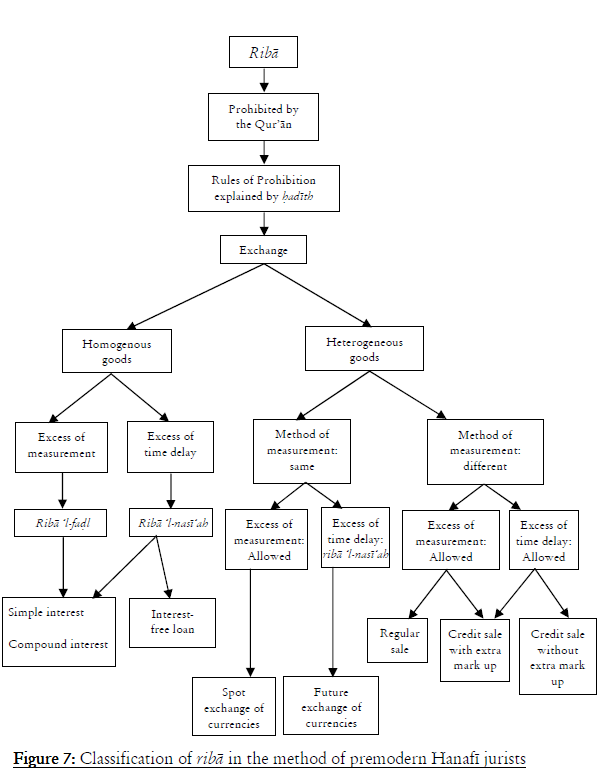
\includegraphics{CourantsIslamContemporain/ImagesCourantsIslamContemporain/Ribadistinction.png}

\end{figure}
L'approche, si elle relativement simple dans sa méthode, est complexe dans son résultat, même pour une personne assez familière des différents concepts financiers. Elle est aussi très rigoriste dans son application : pas de prêt à intérêt, pas d'épargne à taux fixe, limitation du prêt au cadre familial, pas de possibilité de se couvrir sur des marchés à terme,  seule la vente à crédit est autorisée.
 
 Dans l'ensemble, les recherches que nous avons faites en bibliothèque nous ont plutôt orienté vers une application stricte du \riba. 
 
 %--------------------------------------------------------------------------------------------- 
\section{Les nouveaux penseurs et le \riba}
 \paragraph{Une application plus souple dans les faits : l'exemple de Tareq Oubrou} Tareq Oubrou, qui essaye de montrer la malléabilité du droit et qui répond à une question sur l'alcool en mentionnant les banques : 
 \begin{quote}
    On fait parfois les choses par contraintes, mais aussi par courtoisie, parce qu’aussi la courtoisie permet certaines choses. Il y a des limites bien sur, tu ne vas pas, sous prétexte de faire plaisir aux autres, boire du vin, etc. Tu respectes tes valeurs mais tu n’es pas obligé de les imposer aux autres, sinon la vie des musulmans deviendra impossible, impossible. Même les banques, le système économique n’est pas totalement équitable (ndlr : d’un point de vue islamique s’entend, car la ribâ est un principe qui théoriquement interdit l’usure, le prêt à intérêt. Mais dès le début de l’expansion de l’islam les mujtahid ont construit des fictions canoniques qui permettent de contourner l’interdit). Même à l’époque du Prophète la réalité n’est pas parfaite, il y avait beaucoup de formes de l’humain que le Prophète n’a pas interdit parce que c’était impossible, parce que « Si tu veux être obéi ; ordonne le possible » comme dit la sagesse. Même Dieu n’a pas interdit tout, y compris des formes de commerce qui n’étaient pas conforme à la Justice, mais elles étaient ancrées dans les coutumes, que l’islam n’a pas pu interdire parce que ça allait casser tout le système économique et même semer le doute envers la religion. Non ! L’essentiel c’est d’être souple. […]  \sn{\cite{Baylocq:Oubrou}}
 \end{quote}



\paragraph{Repenser la norme} Mohammed Talbi et l'école Tunisienne propose de repenser la shari'a en revenant aux principes :
\begin{quote}
    Il existe
trois principes en islam permettant de faire évoluer le droit et de
l'adapter
à la réalité, 

la \emph{maslaha} c'est-à-dire l'utilité publique, un
concept qui date du II\textsuperscript{e} siècle de l'hégire, 

la
\emph{zharoura}, la nécessité, c'est un principe fort puisqu'il est dit
que "la nécessité rend permis l'interdit" ; 

et les \emph{maqassid}, les
finalités de la loi. 
\end{quote}
D'une certaine façon, il s'inscrit dans une certaine filiation avec Abduh qui insistait sur le sens du \riba.

Pratiquement, Talbi mentionne le \riba dans une interview : 
\begin{quote}
  N. O. – Vous parleriez d’une nouvelle sharia ?

M. Talbi. – Absolument. Cela ne signifie pas qu’il faille tout détruire. Je dis oui au jeûne, à la prière, je dis non au voile. Ma position consiste à dire : Mademoiselle ou Madame, rien ne vous oblige à mettre un foulard sur la tête, sauf si vous êtes chrétienne parce que c’est saint Paul qui le dit. Seulement les chrétiennes, aujourd’hui, l’ont abandonné. Pas un mot dans le Coran sur la femme qui doit couvrir ses cheveux. Que l’on me trouve un seul verset où il y a le mot cheveux (chaar).

Il en va de même pour la question de l’usure, du ribâ. On n’a pas défini cette notion. Il n’y avait pas de banques du temps du Prophète. Ce qui était interdit, c’était l’appauvrissement des gens par la spéculation sur la nourriture. \textit{article du Nouvel observateur - « Seul le Coran oblige » - 2005 - trouvé sur le site \textit{nawaat.org} }  
\end{quote}
 
 

\section{Conclusion}


\paragraph{Face à la nouvelle question de la finance, l'approche classique  du droit musulman parait incapable de proposer un cadre adapté} Il existait à l'époque du Prophète un embryon de finance, avec probablement beaucoup d'excès, excès à l'origine de l'interdiction forte du \riba et du \gharar. L'imprécision du terme \riba et les besoins de l'époque de certaines opérations à terme ont entraîné une jurisprudence nombreuse transcrites dans les hadiths puis dans la pensée des différentes écoles juridiques. Cette jurisprudence était adaptée à l'époque,  mais correspond à une économie faiblement capitalisée. Ce cadre paraît aujourd'hui  en inadéquation avec les outils financiers modernes et généralisés comme l'emprunt immobilier (qui peut acheter une maison sans s'endetter ?) ou l'assurance auto (avec le risque de dommage corporel extrêmement lourd, un accident pouvant coûter en Europe plus de 5 millions d'Euro, une somme que seule une mutualité importante de plusieurs milliers de personnes peut soutenir).  

\paragraph{\textit{la nécessité rend permis l'interdit}} Même en Arabie Saoudite, l'assurance auto a été généralisée, au risque d'une certaine schizophrénie des musulmans pratiquants.

\paragraph{une approche d'Abduh pragmatique mais finalement pas suivi} L'approche d'Abduh d'autoriser intérêt et assurance n'a finalement pas été suivie, probablement par le fort développement de la tendance hanbalo-wahhabite en Arabie Saoudite, les hanbalites assimilant \riba à intérêt et \gharar à assurance. En ce sens, après ce travail, la coupure nous semble être entre Abduh (et Oubrou) d'une part et Rida de l'autre, non pas sur les conclusions (ils soutiennent la liceité du prêt à intérêt et de l'assurance) mais dans la justification :  la justification d'Abduh et d'Oubrou est d'abord pragmatique Mais cette approche que l'on pourrait qualifier de \textit{"pastorale"} doit être complétée par une approche théologique renouvelée. C'est ce que propose Rida, par une analyse textuelle des utilisation du \riba dans le Coran et le Hadith. Mais la référence aux Hadiths et aux corpus juridiques classiques pour répondre à une question contemporaine, peut aussi être retournée par des juristes tenants d'une lecture traditionaliste, comme le montre le travail de Siddique. Avec le risque de perdre une partie de sa pertinence en tant que religion, en reprenant la définition de Lindbeck. En ce sens, l'approche de Mohammed Talbi et l'école Tunisienne parait plus adaptée à une réponse féconde sur ces questions.


\paragraph{Le cadre de la vente à terme qui montre ses limites pour analyser les contrats financiers} Les contrats d'assurance et les contrats financiers (prêt), sont analysés par les jurisconsultes dans le cadre classique de la vente de biens à terme. Ces contrats étaient fortement encadrés historiquement pour éviter les sources de conflit futur, liée à l'incertitude de façon générale, incertitude sur le bien (\gharar) ou incertitude sur le niveau d'intérêt (\riba). L'approche financière a repoussé les limites de l'incertitude, en identifiant un certain nombre de domaines (risque d'assurance, risque d'intérêt, ....) où la survenance d'une perte financière a une existence objective qui peut être mesurée et représentée statistiquement. Ces domaines où le risque est \textit{maîtrisé} et où un contrat peut être mis en place, sont donc ceux où \textit{l'incertitude est connue}\sn{les \textit{known-unknowns} selon la définition de D. Rumsfeld}. Dès que l'incertitude n'est pas connue (\textit{unknown-unknown}), aucun contrat ne peut être être établi. \cite{Rittenberg:Gharar} montre la proximité d'une telle approche avec celle des jurisconsultes, essayant quant à eux de définir les conditions où l'incertitude dans l'établissement du contrat peut être maîtrisée. Par cette analogie plus large, il doit être possible d'évaluer théologiquement ces nouveaux contrats dans un cadre plus large que celui de la vente à terme, en intégrant leur utilité sociale et économique.


\subsection{Parallèle potentiellement enrichissant du Christianisme}
\paragraph{Une interdiction historique du prêt à intérêt en Occident} Historiquement, le christianisme connut une réflexion assez parallèle que celle de l'Islam. Ainsi, le Concile de Tours de 1163 condamna le prêt à intérêt. Cette interdiction a même pour soutien une parole de Jésus : 
\begin{quote}
    Mais aimez vos ennemis, faites du bien, \textit{et prêtez sans rien attendre}. Et votre récompense sera grande, et vous serez fils du Très-Haut, car il est bon pour les ingrats et pour les méchants." (Lc 6, 35)
\end{quote}
Cependant, cette interdiction avec le temps disparut, en particulier par une réflexion universitaire à partir de S. Thomas d'Aquin.
 
\paragraph{S. Thomas d'Aquin et l'usure : une réflexion autonome de la théologie}  La réflexion de S. Thomas sur l'usure se révéla particulièrement féconde, à la fois sur la méthode et sur le résultat. Sur la méthode, la réflexion scolastique s'appuie sur la philosophie (ou l'économie), comme ancillaire à la théologie mais comme des \textsc{ disciplines autonomes}. Cette autonomie est essentielle pour permettre à ces disciplines de se développer, de chercher des solutions indépendamment de la norme religieuse; ces développements permettant \textit{in fine} de sortir de certaines impasses théologico-juridiques. 

Sur le fond, Saint Thomas a développé la notion de \textit{juste prix} :
\begin{quote}
    \textit{ Si aliquis carius velit vendere res suas quam sit justum pretium… manifeste usura committitur.} Si quelqu’un veut vendre ses biens plus cher que le juste prix, l’usure est évidente  Thomas d’Aquin, Summa theologica, IIa IIae, quest. LXXVIII
\end{quote}

L'usure, par opposition au juste prix, c'est donc  de proposer pour le même \textit{bien} deux prix différents pour deux personnes différentes ou de dissimuler une information importante sur le bien échangé \sn{\cite{Sivery:UsureThomasAquin}}. Dans ce cadre, on peut dire qu'il existe un juste prix pour un prêt, qui est l'\textit{intérêt} en dehors de toute \emph{usure}. Et de même, il existe  un juste prix pour un risque, qui est le prix actuariel\sn{Le prix actuariel est le prix découlant des statistiques du risque}, en dehors de tout \gharar. 

Il ne s'agit pas ici de conclure que le \textit{juste prix} est La solution pour l'Islam mais d'ouvrir des pistes pour sortir de la situation actuelle de fait d'une interdiction formelle qui n'est pas appliquée en pratique.

